% !TeX encoding = utf8

\documentclass{thesis}

% Додаткові пакети вносьте у цей файл
%%% У даний файл додавайте всі необхідні вам додаткові пакети, наприклад...

\usepackage[h]{esvect} % пакет для символу вектора \vv{x}

\usepackage{xstring} % For string manipulation

% \usepackage{float}

% \usepackage{hyperref}

\usepackage{pdfpages}

\usepackage{caption}

\usepackage{lastpage}

% Додаткові визначення та перевизначення команд вносьте у цей файл
%%% У даному файлі визначайте всі необхідні вам нові команди TeX
%%% Або робіть перевизначення існуючих, наприклад...

% Перевизначення символу порожньої множини та знаків "більше-дорівнює", "менше-дорівнює" на прийняті у нас
\let\oldemptyset\emptyset
\let\emptyset\varnothing
\let\geq\geqslant
\let\leq\leqslant

% Визначення нових математичних команд
\newcommand*{\binsp}[1]{\ensuremath \left\{0, 1\right\}^{#1}}       % {0, 1}^m
\newcommand*{\xor}{\ensuremath \oplus}                              % \xor = (+)
\newcommand*{\GF}[1]{\ensuremath \mathbb F_{#1}}                    % F_n
\newcommand*{\GFgroup}[1]{\ensuremath \mathbb F^{*}_{#1}}           % F^*_n
\newcommand*{\Zring}[1]{\ensuremath \mathbb Z_{#1}}                 % Z_n
\newcommand*{\Zgroup}[1]{\ensuremath \mathbb Z^{*}_{#1}}            % Z^*_n
\newcommand*{\Jset}[1]{\ensuremath \mathbb J_{#1}}                  % J_n
\newcommand*{\Qset}[1]{\ensuremath \mathbb Q_{#1}}                  % Q_n
\newcommand*{\PQset}[1]{\ensuremath \widetilde{\mathbb Q}_{#1}}     % Q~_n
\newcommand*{\cyclic}[1]{\ensuremath \left\langle {#1} \right\rangle} % <g>
\newcommand*{\Legendre}[2]{\ensuremath \left( \frac{#1}{#2} \right)} % символ Лежандра/Якобі
\newcommand*{\compinv}[1]{\ensuremath {#1}^{\left\langle -1 \right\rangle}} % обернений за композицією

% Інший спосіб визначення математичного оператору
\DeclareMathOperator{\ord}{ord}
\DeclareMathOperator{\lcm}{lcm}
\DeclareMathOperator{\Li}{Li}
\DeclareMathOperator{\Coef}{Coef}
\DeclareMathOperator{\Log}{Log}
\DeclareMathOperator{\Exp}{Exp}
\DeclareMathOperator{\Res}{Res}
\DeclareMathOperator{\charact}{char}
\DeclareMathOperator{\Sym}{Sym}

%%% ...і таке інше

% Відомості про автора роботи
%%% Основні відомості %%%

\newcommand{\UDC}{(Внесіть правильний УДК!)} % УДК
% УДК виглядає приблизно як 004.056.5 або 513.2, або навіть 004.056.5:513.2+519.1
% Для того, щоб знайти правильний УДК, використовуйте каталог https://teacode.com/online/udc/

\newcommand{\reportAuthor}             % ПІБ автора повністю
{Омельченко Іван Юрійович}
\newcommand{\reportAuthorGen}          % ПІБ автора в родовому відмінку
{Омельченку Івану Юрійовичу}
\newcommand{\reportAuthorGroup}        % група автора
{КМ-51мп}
\newcommand{\reportTitle}              % Назва роботи
{Автоматична ідентифікація музичних інструментів в аудіозаписах з використанням методів машинного навчання}
%% використовуйте символ "\par" або "\\" для розбиття назви на декілька рядків

\newcommand{\supervisorFio}            % Науковий керівник, ПІБ повністю
{Лось Валерій Миколайович}
\newcommand{\supervisorRegalia}        % Науковий керівник: посада, степінь, звання
{професор кафедри ПMA, доктор фіз.-мат. наук}              % наприклад: доцент кафедри ПМА, канд. техн. наук, доцент

\newcommand{\reportOrder}{\quotes{29} травня 2025 р. \No 1808-С} % реквізити наказу

\newcommand{\applicationDate}          % термін подання роботи
{\quotes{10} червня 2025 р.}

\newcommand{\assignmentDate}           % дата видачі завдання
{\quotes{03} лютого 2025 р.}

% Якщо у вас нема консультанта - залишайте поля нижче порожніми
\newcommand{\consultFio}               % Консультант, ПІБ повністю
{Прізвище Ім'я По батькові}
\newcommand{\consultRegalia}           % Консультант: звання, ступінь, посада
{посада, ступінь, звання}

\newcommand{\reviewerFio}              % Рецензент, ПІБ повністю
{---}                        
\newcommand{\reviewerRegalia}          % Рецензент: звання, ступінь, посада
{---}

\newcommand{\consultdstuFio}           % Консультант з нормоконтролю, ПІБ повністю
{Мальчиков Володимир Вікторович}                        
\newcommand{\consultdstuRegalia}       % Консультант з нормоконтролю: звання, ступінь, посада
{старший викладач кафедри ПМА}

\newcommand{\YearOfDefence}            % рік захисту
{2026}
\newcommand{\YearOfBeginning}          
{2026}



% ************************************************************* %
% Обробка даних
% ************************************************************* %

\newcommand{\takeSecondFIRST}[1]{%
    \StrBefore{#1}{ }[\FirstWord]% Extract the first word
    \StrBehind{#1}{ }[\Rest]% Extract the rest after the first word
    \StrBefore{\Rest}{ }[\SecondWord]% Extract the second word
    \StrBehind{\Rest}{ }[\ThirdWord]% Extract the third word
    \SecondWord\ \MakeUppercase{\FirstWord}% Print first word and uppercase second word
}

\newcommand{\supervisorFioShort}{
    \takeSecondFIRST{\supervisorFio}
}
\newcommand{\reportAuthorShort}{
    \takeSecondFIRST{\reportAuthor}
}


% Починаємо верстку документа
\begin{document}

% Створюємо титульну сторінку
\thispagestyle{empty}
\setlength{\parindent}{0cm}

\begin{center}
\textbf{\MakeUppercase{Національний технічний університет України}}

\textbf{\MakeUppercase{\quotes{Київський політехнічний інститут\\ імені Ігоря Сікорського}}}

\textbf{Факультет програмних систем та прикладної математики}

\textbf{Кафедра прикладної математики}

\vfill % автоматично заповнюємо проміжок

{\renewcommand{\arraystretch}{0.8}
\begin{tabularx}{\textwidth}{@{}Xl@{}}
	
& \quotes{До захисту допущено} \\
& Завідувач кафедри \\
& \_\_\_\_\_\_\_\_\_\_\_\_\_~Данило ТАВРОВ \\
& \quotes{\_\_\_\_}~\_\_\_\_\_\_\_\_\_\_\_\_\_~\the\year~р. \\

\end{tabularx}}

\vfill % автоматично заповнюємо проміжок

\linespread{1.2}
\setfontsize{20}
\textbf{{Магістерська дисертація}}
\setfontsize{14}

\textbf{на здобуття ступеня магістра}

\textbf{за освітньо-науковою програмою \quotes{Наука про дані та математичне \\моделювання}}

\textbf{зі спеціальності \quotes{Прикладна математика}}

\textbf{на тему: \quotes{\reportTitle}}
\linespread{1.5}

\end{center}

\vfill % автоматично заповнюємо проміжок

{\renewcommand{\arraystretch}{0.7}
\begin{tabularx}{\textwidth}{>{\setlength\hsize{1.5\hsize}}X >{\setlength\hsize{0.5\hsize}}X}
Виконав:                                                 & \\
студент групи \reportAuthorGroup               			 & \\
\reportAuthor                                            & \rule{2.5cm}{0.25pt}   \\[6pt]
Керівник:                                                & \\
\supervisorRegalia                                       & \\
\supervisorFio                                           & \rule{2.5cm}{0.25pt}   \\[6pt]
%%% Якщо у вас є консультант у роботі - розкоментуйте наступні три рядки (а цей - не розкоментовуйте!)
% Консультант:                                             & \\
% \consultRegalia,                                         & \\
% \consultFio                                              & \rule{2.5cm}{0.25pt}   \\[6pt]
Консультант з нормоконтролю:                             & \\
\consultdstuRegalia                                      & \\
\consultdstuFio                                          & \rule{2.5cm}{0.25pt}   \\[6pt]
Рецензент:                                               & \\
\reviewerRegalia                                         & \\
\reviewerFio                                             & \rule{2.5cm}{0.25pt} 
\end{tabularx}}

\vfill % автоматично заповнюємо проміжок

\begin{flushright}
	\renewcommand{\arraystretch}{0.8}
	\begin{tabular}{l}
		Засвідчую, що в цій магістерській дисертації\\
		немає запозичень із праць інших авторів\\
		без відповідних посилань.\\
		Студент~\_\_\_\_\_\_\_\_\_\_\_\_\_
	\end{tabular}
\end{flushright}

\vfill % автоматично заповнюємо проміжок

\begin{center}
{Київ~---~\YearOfDefence\ року}
\end{center}

\clearpage % починаємо з нової сторінки

\setcounter{page}{2} % номер сторінки буде 2

\setlength{\parindent}{1.25cm} % задаємо відступ першого рядка абзацу (5 знаків, або 1.25 см)

% пропуск рядка до та після формули
\setlength{\belowdisplayskip}{14pt}
\setlength{\abovedisplayskip}{14pt}
\setlength{\belowdisplayshortskip}{14pt}
\setlength{\abovedisplayshortskip}{14pt}


% Створюємо завдання
\pagestyle{empty}
\setlength{\parindent}{0cm}

{\centering
    \textbf{Національний технічний університет України}

    \textbf{\quotes{Київський політехнічний інститут імені Ігоря Сікорського}}

    \textbf{Факультет прикладної математики}

    \textbf{Кафедра прикладної математики}

}

{\raggedright
Рівень вищої освіти --- другий (магістерський)

Спеціальність --- 113~Прикладна математика

Освітньо-наукова програма \quotes{Наука про дані та математичне моделювання}

}

\addvspace{12pt}

\begin{flushright}
	\renewcommand{\arraystretch}{0.8}
	\begin{tabular}{l}
		\MakeUppercase{Затверджую} \\
		Завідувач кафедри \\
		\_\_\_\_\_\_\_\_\_\_\_\_\_~Данило ТАВРОВ \\
		\quotes{\_\_\_\_}~\_\_\_\_\_\_\_\_\_\_\_\_\_~\the\year~р. \\
	\end{tabular}
\end{flushright}

{\centering
	\textbf{\MakeUppercase{Завдання}}
	
	\textbf{на магістерську дисертацію студенту}

	\reportAuthorGen

}

1. Тема дисертації: \quotes{\reportTitle},
керівник роботи \supervisorFio, \supervisorRegalia, затверджені наказом по університету \reportOrder.

2. Термін подання студентом дисертації: \applicationDate

3. Вихідні дані до роботи: вихідними даними є музичні аудіозаписи у звуковому форматі з відкритого датасету Isophonics, що містить акордові анотації для творів The Beatles у форматі часових міток, а також стандартизовані метрики оцінювання MIREX.

4. Зміст роботи: аналіз існуючих підходів до автоматичного гармонічного аналізу музики; дослідження методів цифрової обробки аудіосигналів (STFT, CQT) та виділення хроматичних ознак; розробка математичної моделі послідовнісної класифікації гармонічних функцій акордів; реалізація та навчання моделі на основі двонапрямленої рекурентної нейронної мережі (BiLSTM); експериментальне оцінювання якості запропонованого методу та порівняння з базовими підходами (HMM, SVM).

5. Перелік ілюстративного матеріалу: концептуальна схема взаємодії компонентів системи автоматичного гармонічного аналізу; графіки динаміки навчання моделі; таблиця порівняння методів автоматичного гармонічного аналізу; таблиця результатів оцінювання моделі на тестовій вибірці.

6. Дата видачі завдання: \assignmentDate

\begin{center}

Календарний план

\addvspace{12pt}

\DefTblrTemplate{firsthead, middlehead, lasthead, firstfoot, middlefoot, lastfoot}{default}{}

\begin{longtblr}{
    hlines,
    vlines,
    colspec = {Q[0.1\textwidth, c] Q[0.4\textwidth, l] Q[0.25\textwidth, c] Q[0.15\textwidth, c]},
    cells = {cmd={\linespread{1.2}\selectfont}},
    rowhead = {1},
    rows = {valign=m},
    row{1} = {halign=c},
}
\No\ з/п & Назва етапів виконання магістерської дисертації & Термін виконання етапів роботи & Примітка \\

1 & Узгодження теми дисертації з науковим керівником, огляд наукових публікацій за тематикою дослідження & ХХ 2025 р. & \\
2 & Аналіз існуючих підходів до автоматичного гармонічного аналізу музики, написання розділу огляду & ХХ 2025 р. & \\
3 & Дослідження методів цифрової обробки аудіосигналів, розробка математичної моделі & ХХ 2025 р. & \\
4 & Реалізація модулів попередньої обробки аудіосигналу та виділення хроматичних ознак & ХХ 2026 р. & \\
5 & Розробка та навчання моделі BiLSTM для послідовнісної класифікації гармонічних функцій & ХХ 2026 р. & \\
6 & Проведення експериментального дослідження, порівняння з базовими методами (HMM, SVM) & ХХ 2026 р. & \\
7 & Написання розділів дисертації, підготовка висновків та списку використаних джерел & ХХ 2026 р. & \\
8 & Остаточне оформлення дисертації, підготовка презентації & ХХ 2026 р. & \\
9 & Подання повної версії магістерської дисертації & ХХ 2026 р. & \\

\end{longtblr}

\vspace{-0.5cm}

\begin{tblr}{
    colspec = {Q[7cm, l] X[c] X[r]},
    cells = {cmd={\linespread{1.2}\selectfont}},
    column{1} = {leftsep=0pt},
    column{Z} = {rightsep=0pt},
}

Студент &  \_\_\_\_\_\_\_\_\_\_\_\_\_ & \reportAuthorShort \\
Керівник роботи & \_\_\_\_\_\_\_\_\_\_\_\_\_ & \supervisorFioShort \\

\end{tblr}

\end{center}

\clearpage
\setlength{\parindent}{1.25cm}

\setlength{\belowdisplayskip}{21pt}
\setlength{\abovedisplayskip}{21pt}
\setlength{\belowdisplayshortskip}{21pt}
\setlength{\abovedisplayshortskip}{21pt}

% Створюємо реферат
%!TEX root = ../thesis.tex
\renewcommand{\abstractUkr}{\chapter*{РЕФЕРАТ}\thispagestyle{empty}\renewcommand{\arraystretch}{1.5}\setfontsize{14}}
\renewcommand{\abstractEng}{\chapter*{ABSTRACT}\thispagestyle{empty}\renewcommand{\arraystretch}{1.5}\setfontsize{14}}


\abstractUkr

Магістерську дисертацію виконано на \pageref{LastPage} аркушах, вона містить перелік посилань на використані джерела з 12 найменувань. У роботі наведено 1 рисунок та 1 таблицю.

\textbf{Актуальність теми.}
Автоматична ідентифікація музичних інструментів в аудіозаписах є
актуальною задачею музичної інформатики, яка знаходиться на перетині
цифрової обробки сигналів і машинного навчання. Визначення складу
інструментів у музичному записі є необхідним для автоматичної
каталогізації, пошуку та аналізу музичних колекцій, а також для
підтримки задач автоматичного аранжування, ремейксування та
реставрації аудіо.

Реальні музичні твори містять одночасне звучання кількох інструментів,
тому задача відноситься до класу multi-label класифікації, де кожному
аудіозапису може відповідати довільна підмножина інструментальних
міток. Застосування сучасних методів глибинного навчання, зокрема
згорткових та рекурентних нейронних мереж, відкриває можливості для
побудови ефективних автоматизованих систем ідентифікації інструментів
безпосередньо на основі аудіосигналу.

\textbf{Мета і задачі дослідження.}
Метою дисертаційної роботи є побудова математичного та програмного
забезпечення методу автоматичної ідентифікації музичних інструментів
у звуковому форматі та дослідження його ефективності для задачі
multi-label класифікації інструментального складу аудіозаписів.

Для досягнення поставленої мети вирішено такі задачі:

а) проведено огляд і порівняльний аналіз існуючих методів автоматичної
ідентифікації музичних інструментів в аудіозаписах;

б) виконано аналіз і порівняння підходів до побудови математичної
моделі методу multi-label класифікації інструментального складу,
обрано оптимальний варіант;

в) побудовано математичну модель методу, що описує повний цикл
перетворення аудіосигналу у вектор інструментальних міток;

г) проведено порівняльний аналіз варіантів конфігурації
запропонованого методу та досліджено його властивості на
стандартизованому наборі даних;

д) виконано порівняння ефективності запропонованого методу з
існуючими підходами.

\textbf{Об'єктом дослідження} є інструментальний склад музичних творів
у звуковому форматі та методи його автоматичної ідентифікації на основі
цифрової обробки сигналів і машинного навчання.

\textbf{Предметом дослідження} є математичне та програмне забезпечення
методу автоматичної ідентифікації музичних інструментів (гітара, фортепіано,
ударні, бас, скрипка тощо) на основі мел-спектрограм аудіосигналу та
гібридної архітектури CNN~+~BiLSTM.

\textbf{Методи дослідження.}
Методи цифрової обробки аудіосигналів (STFT, мел-фільтрбанк), методи
виділення тембральних спектральних ознак (мел-спектрограми, MFCC),
методи multi-label класифікації на основі згорткових і рекурентних
нейронних мереж, методи навчання та оптимізації моделей машинного
навчання, експериментальні методи порівняльного аналізу результатів.

\textbf{Ключові слова:}
ідентифікація музичних інструментів, multi-label класифікація,
машинне навчання, згорткові нейронні мережі, CNN, BiLSTM,
мел-спектрограма, MFCC, бінарна крос-ентропія, F1-міра, mAP,
музична інформатика, IRMAS, тембральний аналіз.

\abstractEng

The master's thesis comprises \pageref{LastPage} pages and includes a list of 12 references. The work contains 1 figure and 1 table.

\textbf{Relevance.}
Automatic identification of musical instruments in audio recordings is
a relevant problem in music information retrieval that lies at the
intersection of digital signal processing and machine learning.
Determining the instrument composition of a musical recording is
essential for automatic cataloguing, search, and analysis of music
libraries, as well as for supporting tasks such as automatic
arrangement, remixing, and audio restoration.

Real-world musical works contain the simultaneous sound of several
instruments, making this a multi-label classification problem where
each audio recording may correspond to an arbitrary subset of
instrument labels. The application of modern deep learning methods,
in particular convolutional and recurrent neural networks, opens
opportunities for building effective automated instrument identification
systems directly from the audio signal.

\textbf{Purpose and objectives.}
The aim of the dissertation is to construct the mathematical and software
support for a method of automatic identification of musical instruments
in audio format and to investigate its effectiveness for the multi-label
classification of the instrument composition of audio recordings.

To achieve this goal, the following tasks were solved:

a) a review and comparative analysis of existing methods for automatic
identification of musical instruments in audio recordings was conducted;

b) an analysis and comparison of approaches to constructing the
mathematical model of the multi-label instrument classification method
was performed, and the optimal variant was selected;

c) a mathematical model of the method was constructed, describing the
full pipeline from audio signal to an instrument label vector;

d) a comparative analysis of configuration variants of the proposed
method was conducted and its properties were investigated on a
standardized dataset;

e) the effectiveness of the proposed method was compared with existing
approaches.

\textbf{Object of research} is the instrument composition of musical
works in audio format and the methods of its automatic identification
based on digital signal processing and machine learning.

\textbf{Subject of research} is the mathematical and software support
for the method of automatic identification of musical instruments
(guitar, piano, drums, bass, violin, etc.) based on mel-spectrograms
of the audio signal and a hybrid CNN~+~BiLSTM architecture.

\textbf{Research methods.}
Methods of digital audio signal processing (STFT, mel filterbank),
methods of timbral spectral feature extraction (mel-spectrograms,
MFCC), methods of multi-label classification based on convolutional
and recurrent neural networks, methods of training and optimization
of machine learning models, experimental methods of comparative
analysis of results.

\textbf{Scientific novelty.}
For the first time, a method for automatic multi-label identification
of musical instruments in audio recordings has been proposed, based on
mel-spectrograms and a hybrid CNN~+~BiLSTM architecture. Unlike
existing approaches focused on single-label recognition or rule-based
filtering, the proposed method directly models the simultaneous
presence of multiple instruments by applying independent sigmoid
activations per class and optimizing binary cross-entropy loss.

\textbf{Practical value.}
Based on the proposed method, software has been implemented that
performs automatic identification of the instrument composition of
musical recordings in audio format. The method has been verified and
validated on the standardized IRMAS dataset, achieving F1-macro and
mAP scores that substantially exceed the results of baseline methods.
The obtained results may be used for the development of applied tools
for music search, automatic annotation, and content-based retrieval
in large audio collections.

\textbf{Keywords:}
musical instrument identification, multi-label classification,
machine learning, convolutional neural networks, CNN, BiLSTM,
mel-spectrogram, MFCC, binary cross-entropy, F1-score, mAP,
music information retrieval, IRMAS, timbral analysis.
\clearpage

\pagestyle{plain}


% Створюємо зміст
% \pagenumbering{gobble}
\tableofcontents
\cleardoublepage
% \pagenumbering{arabic}

% Створюємо перелік умовних позначень, скорочень і термінів
\shortings
%!TEX root = ../thesis.tex
% Cтворюємо перелік умовних позначень, скорочень і термінів у форматі поняття --- розшифровка
% Скорочення потрібно подавати в алфавітному порядку. Скорочення латиницею повинні передувати скороченням кирилицею

%!TEX root = ../thesis.tex
% Cтворюємо перелік умовних позначень, скорочень і термінів у форматі поняття --- розшифровка
% Скорочення потрібно подавати в алфавітному порядку. Скорочення латиницею повинні передувати скороченням кирилицею

ADSR --- Attack, Decay, Sustain, Release --- часова огинаюча звуку: атака, затримка, утримання, спад

BCELoss --- Binary Cross-Entropy Loss --- бінарна крос-ентропійна функція втрат

BiLSTM --- Bidirectional Long Short-Term Memory --- двонапрямлена рекурентна нейронна мережа з довгою короткочасною пам'яттю

CNN --- Convolutional Neural Network --- згорткова нейронна мережа

DCT --- Discrete Cosine Transform --- дискретне косинусне перетворення

GPU --- Graphics Processing Unit --- графічний процесор, використовується для прискорення навчання нейронних мереж

IRMAS --- Instrument Recognition in Musical Audio Signals --- набір даних для розпізнавання інструментів у музичних аудіосигналах

LSTM --- Long Short-Term Memory --- рекурентна нейронна мережа з довгою короткочасною пам'яттю

mAP --- mean Average Precision --- середня точність, стандартна метрика для multi-label класифікації

MFCC --- Mel-Frequency Cepstral Coefficients --- мел-частотні кепстральні коефіцієнти

MIDI --- Musical Instrument Digital Interface --- стандартний протокол цифрового представлення музичних подій

MIREX --- Music Information Retrieval Evaluation eXchange --- міжнародний конкурс оцінювання систем музичної інформатики

ML --- Machine Learning --- машинне навчання

STFT --- Short-Time Fourier Transform --- перетворення Фур'є короткого вікна

SVM --- Support Vector Machine --- метод опорних векторів

МН --- машинне навчання

ОНД --- основи наукових досліджень


% Створюємо вступ
\intro
%!TEX root = ../main.tex

\textbf{Актуальність теми.} Цифрові музичні колекції, потокові сервіси та
архіви звукозаписів містять мільйони творів, для більшості з яких відсутній
опис інструментального складу. Інформація про те, які інструменти звучать у
записі, потрібна для каталогізації та пошуку музики, побудови рекомендаційних
систем, музикознавчого аналізу й навчальних застосунків. Ручне анотування
великих колекцій потребує значних витрат часу фахівців, тому актуальною є
задача автоматичного розпізнавання музичних інструментів у звукових записах.

Найскладнішим є випадок багатоінструментних записів, у яких кілька
інструментів звучать одночасно, їхні спектри накладаються, а набір
присутніх інструментів заздалегідь невідомий. Сучасні підходи на основі
згорткових нейронних мереж суттєво перевершили класичні методи, проте
більшість із них використовують архітектури, запозичені з обробки
зображень, і навчаються на записах з одним переважаючим інструментом, тоді
як застосовуються до багатоінструментних. Крім того, методики оцінювання в
опублікованих роботах часто не описані повністю або передбачають
підбирання налаштувань на тестових даних, що ускладнює чесне порівняння
методів. Отже, актуальним є розроблення моделі, яка враховує тембральну та
часову будову звуку, навчається з урахуванням багатоінструментного
характеру музики та оцінюється за відтворюваною методикою.

\textbf{Метою дослідження} є підвищення точності розпізнавання музичних
інструментів у багатоінструментних звукових записах шляхом розроблення
моделі згорткової нейронної мережі з музично обґрунтованими фільтрами та
методу її навчання на синтетичних сумішах записів.

Для досягнення мети необхідно розв'язати такі \textit{задачі}:
\begin{enumerate}
    \item проаналізувати існуючі методи автоматичного розпізнавання музичних
    інструментів, набори даних і методики оцінювання;
    \item формалізувати задачу багатоміткового розпізнавання інструментів та
    розробити математичну модель розпізнавання: часово-частотне представлення,
    музично обґрунтовані згорткові фільтри, синтез багатоінструментних
    сумішей, правило прийняття рішення;
    \item розробити програмне забезпечення для підготовки даних, навчання,
    розпізнавання та оцінювання моделей;
    \item розробити відтворювану методику оцінювання та провести валідацію
    розробленої моделі на стандартизованому наборі даних, порівнявши її з
    існуючими рішеннями та дослідивши внесок кожної складової моделі.
\end{enumerate}

\textbf{Об'єктом дослідження} є процес автоматичного розпізнавання
музичних інструментів у багатоінструментних звукових записах на основі
згорткових нейронних мереж.

\textbf{Предметом дослідження} є моделі та методи побудови згорткових
нейронних мереж для розпізнавання музичних інструментів, що враховують
тембральну та часову будову звуку.

\textbf{Методи дослідження}: методи цифрової обробки звукових сигналів
(коротковіконне перетворення Фур'є, мел-спектральний аналіз), методи
навчання згорткових нейронних мереж, синтез багатоінструментних сумішей для
розширення навчальних даних та порівняльний експериментальний аналіз
моделей на стандартизованому наборі даних IRMAS з оцінюванням якості за
макро- та мікроусередненою F1-мірою.

\textbf{Наукова новизна} одержаних результатів полягає в такому:
\begin{enumerate}
    \item показано, що на мел-шкалі одна октава займає від трьох до
    двадцяти восьми частотних смуг залежно від висоти, через що вертикальні
    (тембральні) згорткові фільтри сталої висоти охоплюють різні музичні
    інтервали на різних частотах; запропоновано виконувати такі фільтри на
    логарифмічній частотній осі, де кожен фільтр охоплює однаковий музичний
    інтервал незалежно від висоти ноти;
    \item встановлено, що користь явного гармонічного представлення
    (накладання каналів на частотах обертонів) залежить від умов навчання:
    воно покращує розпізнавання при навчанні на записах з одним
    інструментом, але погіршує його при навчанні на синтетичних
    багатоінструментних сумішах;
    \item розроблено модель, яка поєднує музично обґрунтовані фільтри з
    навчанням на синтетичних сумішах і за суворішої методики оцінювання
    перевершує опубліковані результати відомих згорткових моделей на наборі
    даних IRMAS за меншої кількості параметрів.
\end{enumerate}

\textbf{Практичне значення} одержаних результатів полягає в розробленому
програмному забезпеченні, яке може бути використане для автоматичної
каталогізації та пошуку в музичних колекціях, а також як основа для
подальших досліджень тембрового аналізу та змістового музичного пошуку.

%!TEX root = ../main.tex

\chapter{Огляд існуючих рішень з автоматичного розпізнавання музичних інструментів}
\label{chap:review}

Автоматичне розпізнавання музичних інструментів є однією з базових задач
музичного інформаційного пошуку. Вона полягає у визначенні за звуковим
сигналом множини інструментів, що звучать у записі. У цьому розділі
розглянуто фізичну природу тембру, на якій ґрунтується розпізнавання,
типовий спосіб часово-частотного представлення звукового сигналу, основні
класи існуючих методів (від класичних методів на основі ручно
сконструйованих ознак до згорткових нейронних мереж) разом із загальними
прийомами їх навчання та застосування, способи врахування гармонічної
будови звуку, методи розширення навчальних даних, комерційні застосунки, а
також набори даних і методики оцінювання. На основі огляду визначено
недоліки існуючих рішень, які обґрунтовують напрям цієї роботи.

% ------------------------------------------------------------------
\section{Постановка задачі розпізнавання музичних інструментів}
\label{sec:task}

Залежно від характеру вхідних даних розрізняють кілька варіантів задачі.
Найпростішим є розпізнавання \textit{ізольованих нот}, записаних окремо для
кожного інструмента в контрольованих умовах. Складнішим є розпізнавання
\textit{сольних фрагментів}, де інструмент виконує музичну фразу з
характерними прийомами гри. Найбільш наближеним до практики є
розпізнавання інструментів у \textit{багатоінструментних записах}, де
кілька джерел звучать одночасно, їхні спектри перекриваються, а до сигналу
додаються ударні, ефекти обробки та шуми запису~\cite{essid2006,fuhrmann2012}.

У багатоінструментному випадку задача природно формулюється як
\textit{багатоміткова класифікація}: кожному запису відповідає довільна
підмножина з $K$ класів інструментів, а не один клас~\cite{tsoumakas2007}.
Часто розглядають її різновид: розпізнавання \textit{переважаючих}
інструментів, тобто тих, що чітко виділяються у звучанні, без вимоги
знайти всі інструменти суміші~\cite{irmas2012}. Особливістю найпоширенішого
набору даних IRMAS є те, що навчальні фрагменти позначено одним
переважаючим інструментом, а тестові одним або кількома. Отже, модель
навчається на одноміткових даних, а оцінюється на багатоміткових, що є
окремим джерелом складності.

% ------------------------------------------------------------------
\section{Тембр і його акустичні ознаки}
\label{sec:timbre}

Тембр є властивістю звуку, яка дає змогу розрізнити два звуки
однакової висоти та гучності. З фізичного погляду тембр визначається
кількома групами характеристик~\cite{muller2015,herrera2003}.

\textit{Гармонічна будова.} Звук більшості мелодичних інструментів є
квазіперіодичним і містить основний тон частоти $f_0$ та обертони на
частотах, близьких до $h f_0$, $h = 2, 3, \ldots$ Співвідношення амплітуд
обертонів характерне для інструмента: так, у звуці кларнета в нижньому
регістрі парні обертони значно слабші за непарні.

\textit{Спектральна обвідна} є плавною функцією, що описує розподіл
енергії за частотою незалежно від конкретної ноти. Вона формується
резонансами корпусу інструмента чи голосового тракту (формантами).

\textit{Часова обвідна} описує зміну амплітуди звуку в часі: швидкість
атаки, наявність сталої фази та характер згасання. Наприклад, фортепіано та
гітара мають різку атаку і поступове згасання, тоді як орган і смичкові
інструменти можуть звучати рівно протягом тривалого часу.

\textit{Шумові складові} (звуки дихання у духових інструментах, тертя
смичка, удар молоточка) також несуть інформацію про джерело звуку.

Ці характеристики є основою як для ручного конструювання ознак у
класичних методах, так і для обґрунтування архітектурних рішень у
нейромережевих моделях.

% ------------------------------------------------------------------
\section{Часово-частотне представлення звукового сигналу}
\label{sec:tfgen}

Більшість методів розпізнавання інструментів, як класичних, так і
нейромережевих, працюють не безпосередньо зі звуковим сигналом, а з його
часово-частотним представленням~\cite{muller2015,choi2017}. Нижче
описано типовий спосіб його обчислення; наведені значення параметрів
поширені в роботах з розпізнавання інструментів~\cite{han2017}.

\textit{Попередня обробка.} Стереосигнал перетворюють на одноканальний
усередненням каналів, передискретизують до частоти $f_s$ (типово
22\,050~Гц) і нормують за піковою амплітудою~\cite{han2017}:
\begin{equation}
    s(n) \leftarrow \frac{s(n)}{\max_n |s(n)|}.
\end{equation}

\textit{Коротковіконне перетворення Фур'є}~\cite{oppenheim2010,muller2015}.
Сигнал ділять на кадри довжиною $N_w$ відліків з кроком $H$ і для кожного
кадру, помноженого на віконну функцію $w(n)$, обчислюють спектр
\begin{equation}
    X(m, k) = \sum_{n=0}^{N_w-1} s(n + mH)\, w(n)\, e^{-2\pi j k n / N_w},
    \quad k = 0, \ldots, N_w/2,
\end{equation}
де $m$ є номером кадру. При $f_s = 22050$~Гц, $N_w = 1024$ і $H = 512$
кадр триває близько 46~мс, а крок становить близько 23~мс.

\textit{Мел-спектрограма.} Мел-шкала пов'язує частоту $f$ у герцах із
суб'єктивно сприйнятою висотою~\cite{stevens1937}; використовується
поширене наближення~\cite{oshaughnessy1987}:
\begin{equation}
    \mu(f) = 2595 \log_{10}\!\left(1 + \frac{f}{700}\right).
    \label{eq:mel}
\end{equation}
Інтервал $[0;\, f_s/2]$ ділять на $F + 1$ рівних відрізків на мел-шкалі,
і центр $b$-ї смуги
\begin{equation}
    \mu_b = b\, \Delta\mu, \quad \Delta\mu = \frac{\mu(f_s/2)}{F+1},
    \quad b = 1, \ldots, F.
    \label{eq:melcentres}
\end{equation}
Банк трикутних фільтрів $\Phi \in \mathbb{R}^{F \times (N_w/2+1)}$,
запропонований для обчислення мел-частотних ознак~\cite{davis1980},
підсумовує енергію спектра в кожній смузі, а логарифмічна мел-спектрограма
\begin{equation}
    M(b, m) = \ln\!\left( \sum_k \Phi_{bk}\, |X(m,k)|^2 + \varepsilon \right),
    \label{eq:logmel}
\end{equation}
де мала стала $\varepsilon$ (наприклад, $10^{-9}$) запобігає логарифму
нуля.

\textit{Часові похідні.} Для відображення часової обвідної, як і в
класичних динамічних ознаках мовних сигналів~\cite{furui1986},
обчислюють першу та другу центральні різниці вздовж осі часу:
\begin{equation}
    \Delta M(b,m) = \frac{M(b,m+1) - M(b,m-1)}{2}, \qquad
    \Delta^2 M = \Delta(\Delta M).
\end{equation}

Логарифмічна мел-спектрограма, іноді разом із похідними, є найпоширенішим
входом згорткових моделей розпізнавання
інструментів~\cite{han2017,pons2017}.

% ------------------------------------------------------------------
\section{Методи на основі ручно сконструйованих ознак}
\label{sec:classical}

Перші системи розпізнавання інструментів ґрунтувалися на обчисленні
набору ознак, що описують тембр, і подальшій класифікації за допомогою
статистичних моделей~\cite{herrera2003}. Найпоширенішими ознаками є
мел-частотні кепстральні коефіцієнти, що компактно описують спектральну
обвідну~\cite{davis1980}, спектральні ознаки (центроїд, розкид, нахил,
спад спектра), ознаки часової обвідної (тривалість атаки, швидкість
згасання) та ознаки гармонічності. Великий перелік таких ознак
систематизовано в роботі~\cite{peeters2004}.

Як класифікатори використовували суміші гауссових розподілів, метод
опорних векторів та метод $k$ найближчих сусідів~\cite{marques1999,
agostini2003}. Для ізольованих нот і сольних фрагментів такі системи
досягали високої точності~\cite{eronen2000}, проте в багатоінструментних
записах їхня якість різко знижується, оскільки ознаки, обчислені за всім
сигналом, змішують внески кількох джерел. Для подолання цієї проблеми
запропоновано ієрархічні класифікатори на основі автоматично побудованих
таксономій ансамблів~\cite{essid2006}, зважування ознак з урахуванням
ступеня їх перекриття~\cite{kitahara2007}, а також попереднє виділення
переважаючого джерела методами розділення звуку~\cite{irmas2012}.

Саме в роботі~\cite{irmas2012} разом із набором даних IRMAS запропоновано
базовий метод на основі ознак та методу опорних векторів, що досягає
макроусередненої F1-міри $0{,}432$ і мікроусередненої $0{,}503$ на
тестовій частині набору~\cite{pons2017}. Загальним недоліком методів цієї
групи є залежність від експертного вибору ознак, які не завжди
відображають відмінності між близькими за звучанням інструментами.

% ------------------------------------------------------------------
\section{Згорткові нейронні мережі}
\label{sec:cnn}

Згорткові нейронні мережі навчаються виділяти ознаки безпосередньо з
часово-частотного представлення сигналу~\cite{lecun2015,goodfellow2016}.
Як вхід зазвичай використовують логарифмічну мел-спектрограму, тобто
двовимірну матрицю «частота $\times$ час», яку мережа обробляє подібно до
зображення.

\subsection{Мережі загального призначення}

Найвідомішим рішенням для набору IRMAS є модель
Хана, Кіма та Лі~\cite{han2017}. Вона складається з чотирьох блоків по дві
згортки $3 \times 3$ з подальшим підвибором, глобального вибору максимуму
та двох повнозв'язних шарів і має близько 1,45~млн параметрів. Модель
навчається на фрагментах тривалістю 1~с, а під час розпізнавання
тестовий запис обробляється ковзним вікном, оцінки вікон підсумовуються та
нормуються на максимум, після чого застосовується поріг. Автори
повідомляють макроусереднену F1-міру $0{,}503$ та мікроусереднену
$0{,}602$. Водночас, згідно з текстом роботи, тривалість вікна, спосіб
агрегації та поріг обирались за найкращим значенням F1-міри, а окремого
опису перевірочної вибірки для цього вибору не наведено, що робить
результат дещо оптимістичним.

Інші роботи досліджували навчання безпосередньо на звуковому
сигналі~\cite{li2015}, спіральне представлення висоти тону, що враховує
октавну подібність~\cite{lostanlen2016}, спільне розпізнавання
інструментів і висоти тону на рівні окремих кадрів~\cite{hung2018}, а також
механізми уваги для розпізнавання за слабкими мітками на наборі
OpenMIC-2018~\cite{gururani2019,openmic2018}.

\subsection{Мережі з музично обґрунтованими фільтрами}

Пояснення роботи мереж загального призначення ускладнене тим, що квадратні
фільтри не мають очевидного акустичного змісту. Понс та
співавтори~\cite{pons2017} запропонували проєктувати форму фільтрів першого
шару відповідно до будови тембру. \textit{Вертикальні} фільтри охоплюють
велику частину частотної осі в межах одного або кількох кадрів і
відображають спектральну обвідну. Фільтри малої висоти та більшої
ширини відображають часову обвідну. У запропонованій ними моделі для
IRMAS перший шар містить фільтри висотою $5$ і $80$ смуг (із $96$) різної
ширини, після нього виконується підвибір майже за всією частотною віссю,
далі два згорткові шари та повнозв'язний шар. Модель має близько
743~тис. параметрів і досягає макроусередненої F1-міри $0{,}516$ та
мікроусередненої $0{,}589$, тобто кращого за модель~\cite{han2017}
значення макроусередненої міри за вдвічі меншої кількості параметрів. Як
і в роботі~\cite{han2017}, поріг рішення ($0{,}2$) та протокол вибору
моделі детально не обґрунтовано, а кількість незалежних запусків не
вказано.

Висоту таких фільтрів задають у частотних смугах мел-спектрограми. Як буде
показано в розділі~\ref{chap:math}, через нерівномірність мел-шкали
фільтр сталої висоти охоплює різні музичні інтервали на різних частотах,
що суперечить ідеї фільтра, який описує тембр незалежно від висоти ноти.

\subsection{Попередньо навчені моделі}

Окремий напрям становлять моделі, попередньо навчені на великих наборах
загальних звуків, зокрема AudioSet~\cite{gemmeke2017,hershey2017,kong2020},
з подальшим донавчанням на цільовій задачі. Такі моделі зазвичай мають
десятки мільйонів параметрів і досягають вищої якості, проте потребують
значних обчислювальних ресурсів, а їхні результати важко зіставляти з
моделями, навченими лише на цільовому наборі. Тому в цій роботі
розглядаються лише моделі, які навчаються з нуля на наборі IRMAS без
залучення зовнішніх даних.

\subsection{Навчання для багатоміткової класифікації}
\label{sec:traingen}

Для багатоміткової постановки вихідний шар мережі містить $K$ незалежних
сигмоїдних виходів $p_k = \sigma(z_k) = 1/(1 + e^{-z_k})$, кожен з яких
оцінює ймовірність присутності відповідного
інструмента~\cite{tsoumakas2007,goodfellow2016}. Параметри мережі
$\theta$ визначають мінімізацією бінарної перехресної ентропії,
усередненої за класами та прикладами пакета з $B$ прикладів:
\begin{equation}
    \mathcal{L}(\theta) = -\frac{1}{BK} \sum_{i=1}^{B} \sum_{k=1}^{K}
    \Big[ y_{ik} \ln p_{ik} + (1 - y_{ik}) \ln(1 - p_{ik}) \Big].
    \label{eq:bce}
\end{equation}
Для мінімізації поширено використовують метод Adam~\cite{kingma2015}, а
крок навчання поступово зменшують, зокрема за косинусним
законом~\cite{loshchilov2017}:
\begin{equation}
    \eta_e = \eta_{\min} + \frac{1}{2}(\eta_0 - \eta_{\min})
    \left(1 + \cos\frac{\pi e}{E}\right),
    \label{eq:cosine}
\end{equation}
де $e$ позначає номер епохи, $E$ задає кількість епох, а $\eta_0$ і
$\eta_{\min}$ є початковим і кінцевим кроком. Для стабілізації навчання
застосовують пакетну нормалізацію~\cite{ioffe2015}, а для регуляризації
проріджування, тобто випадкове вимикання каналів і нейронів під час
навчання~\cite{srivastava2014}.

\subsection{Розпізнавання записів довільної тривалості}
\label{sec:inference}

Моделі навчають на фрагментах фіксованої тривалості (як правило, 1--3~с),
тоді як записи, що аналізуються, довші. У роботі~\cite{han2017}
запропоновано обробляти запис ковзним вікном довжиною $T$ кадрів з кроком
$T/2$, обчислювати для вікон $w = 1, \ldots, W$ ймовірності
$\mathbf{p}^{(w)}$ та агрегувати їх підсумовуванням з нормуванням на
максимум:
\begin{equation}
    S_k = \sum_{w=1}^{W} p^{(w)}_k, \qquad
    \bar{S}_k = \frac{S_k}{\max_{j} S_j}.
    \label{eq:s2}
\end{equation}
Нормування гарантує, що найвпевненіше розпізнаний інструмент отримує
оцінку 1. Остаточне рішення приймається за порогом $\tau$:
\begin{equation}
    \hat{y}_k =
    \begin{cases}
        1, & \bar{S}_k \geq \tau, \\
        0, & \bar{S}_k < \tau,
    \end{cases}
    \qquad k = 1, \ldots, K.
    \label{eq:decision}
\end{equation}
Автори~\cite{han2017} порівнювали також усереднення оцінок без нормування
й обрали нормоване підсумовування з порогом $0{,}5$; у
роботі~\cite{pons2017} оцінки усереднюються, а поріг становить $0{,}2$.

% ------------------------------------------------------------------
\section{Гармонічні та частотно-інваріантні представлення}
\label{sec:harmonic}

Мел-спектрограма має нерівномірну частотну роздільність: смуги рівномірно
розташовані на психоакустичній мел-шкалі~\cite{stevens1937}, яка є майже
лінійною нижче 1~кГц і майже логарифмічною вище. Альтернативою є
перетворення зі сталою добротністю~\cite{brown1991}, у якому кожна октава
містить однакову кількість частотних смуг. На такій осі зміна висоти ноти
відповідає зсуву спектра на сталу кількість смуг, а відстані між
обертонами не залежать від висоти основного тону.

Цю властивість використовують для явного врахування гармонічної будови
звуку. У гармонічному представленні~\cite{bittner2017} кілька копій
спектра, розтягнутих у $h$ разів по частоті, накладаються як канали входу
мережі, так що в одній точці згортка «бачить» енергію основного тону та
обертонів. У роботі~\cite{won2020} запропоновано навчувані гармонічні
фільтри. Інший підхід полягає в розділенні сигналу на гармонічну та ударну
складові методом медіанної фільтрації~\cite{fitzgerald2010}, що дає змогу
зменшити вплив ударних інструментів, які в наборі IRMAS не розмічаються.
Ці представлення здебільшого досліджувались для оцінювання висоти тону та
загальної класифікації звуків, а їхня ефективність для розпізнавання
інструментів у багатоінструментних записах залишається недостатньо
вивченою.

% ------------------------------------------------------------------
\section{Методи розширення навчальних даних}
\label{sec:augmentation}

Набори даних для розпізнавання інструментів невеликі за обсягом, тому
поширеним прийомом є штучне розширення навчальної вибірки. Для звукових
даних застосовують зміну висоти та темпу, додавання шуму, маскування
частотних смуг і часових інтервалів~\cite{park2019,schluter2015}.
Метод змішування прикладів~\cite{zhang2018} формує лінійні комбінації
пар прикладів і їхніх міток, проте для звуку така комбінація логарифмічних
спектрограм не відповідає фізичному додаванню сигналів, а дробові мітки
не відповідають багатомітковій постановці.

Для задачі, в якій навчальні дані містять один переважаючий інструмент, а
тестові кілька, природним є створення штучних
багатоінструментних сумішей з навчальних записів. Такий підхід
досліджувався в роботі~\cite{kratimenos2021}, де показано його користь для
класифікації інструментів у поліфонічній музиці. Водночас питання про те,
як синтетичні суміші взаємодіють з архітектурними рішеннями, зокрема з
гармонічними представленнями, залишається відкритим.

% ------------------------------------------------------------------
\section{Комерційні застосунки}
\label{sec:commercial}

Автоматичне розпізнавання інструментів уже використовується в
комерційних продуктах, як правило, як частина ширших функцій. Сервіси
автоматичного тегування музичних каталогів, зокрема Cyanite~\cite{cyanite},
визначають для записів набір ознак, серед яких жанр, настрій, темп та
інструментальний склад; такі ознаки використовують звукозаписні компанії,
видавці та бібліотеки музики для пошуку й добору творів. Подібні
технології автоматичного тегування та пошуку розвивала компанія Musiio,
яку у 2022~р. придбав сервіс SoundCloud для покращення пошуку
музики~\cite{musiio2022}.

У програмах для зведення звуку розпізнавання інструмента використовується
для автоматичного налаштування обробки: модуль Track Assistant засобу
iZotope Neutron визначає тип інструмента на доріжці (вокал, гітара, бас,
ударні, фортепіано) і пропонує відповідні налаштування~\cite{izotope}.
Близькою задачею є розділення готового запису на складові окремих
інструментів, реалізоване, зокрема, у функції Stem Splitter програми
Logic Pro, яка виділяє вокал, ударні, бас, гітару та
фортепіано~\cite{logicpro2025}.

Спільною рисою комерційних рішень є закритість: методи, навчальні дані
та показники якості, як правило, не публікуються, а набір розпізнаваних
категорій обмежений. Частина рішень працює з окремими доріжками, на яких
звучить один інструмент, а не з готовими багатоінструментними записами.
Тому для порівняння методів використовують відкриті набори даних і
опубліковані результати, розглянуті нижче.

% ------------------------------------------------------------------
\section{Набори даних і методики оцінювання}
\label{sec:datasets}

\textit{IRMAS}~\cite{irmas2012} є стандартним набором даних для
розпізнавання переважаючих інструментів. Він містить 11 класів
(віолончель, кларнет, флейта, акустична гітара, електрогітара, орган,
фортепіано, саксофон, труба, скрипка, голос). Навчальна частина складається
з 6705 фрагментів тривалістю 3~с, вирізаних з понад 2000 записів і
позначених одним переважаючим інструментом; для частини фрагментів у назві
файлу вказано жанр і наявність ударних. Тестова частина містить 2874
фрагменти тривалістю 5--20~с з одним або кількома позначеними
інструментами. Детальніше набір описано в розділі~\ref{sec:data}.

\textit{OpenMIC-2018}~\cite{openmic2018} містить близько 20~тис.
десятисекундних фрагментів з 20 класами та частковою (слабкою)
розміткою. \textit{NSynth}~\cite{engel2017} містить понад 300~тис.
ізольованих нот і придатний переважно для задачі розпізнавання окремих
звуків.

Для оцінювання багатоміткового розпізнавання використовують точність,
повноту та F1-міру для кожного класу, а також їх макроусереднення (середнє
за класами) та мікроусереднення (обчислення за об'єднанням усіх
рішень)~\cite{sokolova2009}. Макроусереднена міра однаково враховує всі
класи, тому чутлива до якості розпізнавання рідкісних інструментів.

Аналіз опублікованих робіт показує, що методики оцінювання на IRMAS
суттєво різняться і часто описані неповно: не завжди вказано спосіб
формування перевірочної вибірки, правило вибору порогу та кількість
незалежних запусків. Окремою проблемою є те, що навчальні фрагменти IRMAS
вирізано з довших записів по кілька з кожного, тому випадковий поділ
фрагментів на навчальну та перевірочну вибірки призводить до потрапляння
частин одного запису в обидві вибірки і завищеної оцінки якості на
перевірочних даних.

% ------------------------------------------------------------------
\section{Висновки до розділу}
\label{sec:ch1_conclusions}

У розділі розглянуто існуючі рішення задачі автоматичного розпізнавання
музичних інструментів. Узагальнене порівняння основних груп методів
наведено в таблиці~\ref{tab:review}.

\begin{table}[H]
\centering
\caption{Порівняння груп методів розпізнавання музичних інструментів}
\label{tab:review}
\small
\begin{tabular}{|p{3.4cm}|p{4.6cm}|p{4.6cm}|p{2.6cm}|}
\hline
\textbf{Група методів} & \textbf{Переваги} & \textbf{Недоліки} &
\textbf{Макро-F1 на IRMAS} \\
\hline
Ручно сконструйовані ознаки та класифікатори~\cite{irmas2012} &
Інтерпретованість, невеликі вимоги до обчислень &
Залежність від вибору ознак, низька якість у сумішах &
0,432 \\
\hline
Згорткові мережі загального призначення~\cite{han2017} &
Автоматичне виділення ознак &
Велика кількість параметрів, відсутність акустичного змісту фільтрів &
0,503 \\
\hline
Мережі з музично обґрунтованими фільтрами~\cite{pons2017} &
Менша кількість параметрів, інтерпретованість фільтрів &
Висота фільтрів задана в мел-смугах, а не в музичних інтервалах &
0,516 \\
\hline
Попередньо навчені моделі~\cite{kong2020} &
Висока якість завдяки великим зовнішнім даним &
Десятки мільйонів параметрів, складність порівняння &
- \\
\hline
Комерційні сервіси~\cite{cyanite,izotope} &
Готові до використання, працюють з великими каталогами &
Закриті методи та показники якості, обмежений набір категорій &
- \\
\hline
\end{tabular}
\end{table}

За результатами огляду виявлено такі недоліки існуючих рішень:
\begin{enumerate}
    \item вертикальні фільтри, що мають описувати тембр, задаються сталою
    висотою в смугах мел-спектрограми і через нерівномірність мел-шкали
    охоплюють різні музичні інтервали на різних частотах;
    \item моделі навчаються на записах з одним переважаючим інструментом, а
    застосовуються до багатоінструментних, причому цю розбіжність, як
    правило, не компенсують на етапі навчання;
    \item вплив явних гармонічних представлень на розпізнавання
    інструментів у сумішах, особливо в поєднанні з розширенням даних,
    недостатньо досліджено;
    \item методики оцінювання на наборі IRMAS неоднорідні: поріг рішення
    іноді обирають за результатами на тестових даних, кількість запусків
    не вказують, а випадковий поділ фрагментів спричиняє перетин
    навчальної та перевірочної вибірок.
\end{enumerate}

Отже, у роботі доцільно розробити модель згорткової нейронної мережі, у
якій тембральні фільтри охоплюють сталі музичні інтервали, навчати її на
синтетичних багатоінструментних сумішах, дослідити роль гармонічних
представлень та оцінювати результати за відтворюваною методикою без
використання тестових даних для вибору налаштувань.

\chapter{Огляд існуючих методів автоматичної ідентифікації
музичних інструментів}
\label{chap:review}

Автоматична ідентифікація музичних інструментів в аудіозаписах є
складною науково-практичною задачею, що перебуває на перетині теорії
музики, цифрової обробки сигналів і машинного навчання. Тембр
інструментів визначає унікальний характер їх звучання та є ключовою
характеристикою для ідентифікації. На відміну від висоти звуку чи
ритму, тембральні властивості визначаються складним поєднанням
спектральних і часових характеристик аудіосигналу.

Складність автоматичної ідентифікації зумовлена кількома чинниками.
По-перше, у реальних записах кілька інструментів звучать одночасно,
утворюючи акустичну суміш, з якої необхідно виокремити окремі тембри.
По-друге, один і той самий інструмент може звучати по-різному залежно
від виконавця, прийому гри та акустики приміщення. По-третє, задача є
multi-label за своєю природою: кожному запису може відповідати довільна
підмножина інструментальних міток, що суттєво ускладнює вибір і
навчання моделі.

У науковій літературі запропоновано різні підходи до автоматичної
ідентифікації музичних інструментів. У цьому розділі розглянуто наявні
підходи як існуючі рішення у галузі музичної інформатики з метою
обґрунтування вибору методів, що застосовуються у даній роботі.

% ------------------------------------------------------------------
\section{Тембральні характеристики музичних інструментів}
\label{sec:timbre_theory}

Тембр є комплексною перцептивною характеристикою звуку, що відрізняє
один інструмент від іншого за однакової висоти та гучності. Фізично
тембр визначається спектральною огинаючою сигналу, часовою динамікою
амплітуди (атака, затримка, утримання, спад --- ADSR) та наявністю
шумових складових~\cite{muller2015}.

Спектральні характеристики інструментів суттєво відрізняються:
\begin{itemize}
    \item струнні інструменти (скрипка, гітара) мають багатий
    обертоновий спектр з характерними резонансними частотами;
    \item духові інструменти характеризуються специфічними формантними
    областями;
    \item ударні інструменти мають шумоподібний спектр з короткою
    атакою та швидким затуханням.
\end{itemize}

Мел-спектрограма є стандартним представленням для аналізу тембру,
оскільки логарифмічна мел-шкала частот відповідає слуховому
сприйняттю людини та добре відображає спектральні відмінності між
інструментами~\cite{piston1987}.

% ------------------------------------------------------------------
\section{Rule-based підходи до ідентифікації інструментів}
\label{sec:rule_based}

Ранні підходи до ідентифікації інструментів ґрунтувалися на
формалізації знань про тембральні характеристики кожного інструменту.
Вони передбачали ручне конструювання ознак --- центроїд спектру,
спектральний розкид, нульові переходи --- та їх порівняння з
наперед визначеними шаблонами або порогами.

Rule-based методи добре працюють для ізольованих інструментів у
контрольованих умовах. Проте вони є чутливими до акустичних умов
запису, не враховують варіацій виконавської техніки та погано
узагальнюються на суміші інструментів. У задачі multi-label
класифікації такі підходи потребують окремого ансамблю детекторів
для кожного інструменту, що ускладнює реалізацію.

% ------------------------------------------------------------------
\section{Класичні методи машинного навчання}
\label{sec:classical_ml}

Застосування класичних методів машинного навчання --- Gaussian Mixture
Models (GMM), метод опорних векторів (SVM), k-найближчих сусідів (kNN)
--- суттєво підвищило якість ідентифікації порівняно з rule-based
підходами. Такі методи навчаються автоматично розрізняти інструменти на
основі наборів спектральних і часових ознак~\cite{ellis2007}.

Для multi-label задачі класичні ML-методи адаптуються через підходи
«один проти одного» або «один проти всіх», де для кожного інструменту
навчається окремий бінарний класифікатор. Серед ознак
широко застосовуються MFCC, спектральний центроїд, спектральний потік
та мел-спектральні коефіцієнти.

Обмеженням класичних ML-методів є те, що вони обробляють кожен фрагмент
незалежно та не здатні враховувати часовий контекст звучання
інструментів. Крім того, якість результатів суттєво залежить від
ручного конструювання ознак.

% ------------------------------------------------------------------
\section{Методи цифрової обробки сигналів}
\label{sec:dsp}

Ключовим етапом будь-якого підходу до ідентифікації інструментів є
виділення інформативних ознак з аудіосигналу. Методи цифрової обробки
забезпечують перехід від сирого аудіосигналу до компактного
представлення, що зберігає тембральну інформацію.

Перетворення Фур'є короткого вікна (STFT) є базовим інструментом
часово-частотного аналізу. На його основі будується мел-спектрограма
--- часово-частотне представлення з мел-шкалою частот, що
відповідає особливостям людського слуху. Мел-частотні кепстральні
коефіцієнти (MFCC) є компактним описом спектральної огинаючої та
широко використовуються для представлення тембру~\cite{harte2006}.

Порівняно з хроматичними ознаками, що застосовуються у гармонічному
аналізі, мел-спектрограми та MFCC є більш інформативними для задачі
ідентифікації тембру, оскільки зберігають інформацію про весь
спектр сигналу, а не лише про клас висоти звуку.

% ------------------------------------------------------------------
\section{Згорткові нейронні мережі (CNN)}
\label{sec:cnn}

Згорткові нейронні мережі продемонстрували високу ефективність у
задачах аналізу зображень і були успішно адаптовані для обробки
спектральних представлень аудіосигналу. Мел-спектрограма природно
інтерпретується як двовимірний образ, де осі відповідають часу та
частоті, що дозволяє застосовувати стандартні CNN-архітектuri для
виявлення тембральних патернів~\cite{korzeniowski2017}.

Двовимірні згорткові фільтри здатні автоматично виявляти локальні
часово-частотні закономірності, характерні для конкретних
інструментів: атакові транзієнти ударних, гармонійні смуги струнних,
формантні структури духових. Операція пулінгу забезпечує інваріантність
до малих зсувів у часі та частоті, підвищуючи стійкість до виконавських
варіацій.

% ------------------------------------------------------------------
\section{Рекурентні нейронні мережі та гібридні архітектури}
\label{sec:rnn}

Рекурентні нейронні мережі, зокрема BiLSTM, дозволяють враховувати
часовий контекст звучання інструментів~\cite{hochreiter1997}. Для задачі
ідентифікації інструментів це важливо, оскільки тембральний образ
інструменту проявляється протягом певного часового проміжку: атака,
утримання та спад є складовими, що разом визначають впізнаваний тембр.

Гібридні архітектури CNN~+~LSTM (або CNN~+~BiLSTM) поєднують
можливості CNN для виявлення локальних тембральних патернів зі
здатністю рекурентних мереж моделювати часові залежності. Такий підхід
є природним для задачі ідентифікації інструментів, де необхідно
враховувати як спектральну структуру (тембр), так і динаміку звучання
у часі~\cite{bock2012}.

% ------------------------------------------------------------------
\section{Огляд існуючих наборів даних та інструментів оцінювання}
\label{sec:datasets}

Для об'єктивного порівняння методів автоматичної ідентифікації
інструментів застосовуються стандартизовані набори даних з розміченими
інструментальними анотаціями.

\subsection{IRMAS}
\label{subsec:irmas}

Датасет IRMAS (Instrument Recognition in Musical Audio Signals)~\cite{irmas2012}
містить близько 6000 тризекундних фрагментів аудіозаписів з анотаціями
для 11 класів інструментів: гітара, електрогітара, орган, фортепіано,
труба, скрипка, гітара-флейта, флейта, ударні, контрабас та голос.
Набір розроблено спеціально для задачі ідентифікації інструментів у
полімодальних записах і є стандартним бенчмарком у галузі.

\subsection{OpenMIC-2018}
\label{subsec:openmic}

OpenMIC-2018~\cite{openmic2018} містить близько 20\,000 десятисекундних
кліпів із слабкими анотаціями для 20 класів інструментів. Слабка
анотація означає, що мітки отримано частково за допомогою краудсорсингу
та не гарантують повноти: відсутність мітки не означає відсутності
інструменту у записі. Це робить набір більш реалістичним, проте
потребує спеціальних підходів до навчання.

\subsection{Метрики оцінювання}
\label{subsec:metrics}

Для оцінювання якості методів multi-label класифікації застосовуються
метрики, що враховують помилки на рівні окремих міток. F1-macro
обчислюється як незважене середнє F1-міри по всіх класах, F1-micro
--- як F1-міра по об'єднаній множині всіх міток. Середня точність
mAP (mean Average Precision) є стандартною метрикою для задач з
нерівномірним розподілом класів і вимірює якість ранжування передбачених
міток.

% ------------------------------------------------------------------
\section{Висновки до розділу}
\label{sec:ch2_conclusions}

У розділі проведено огляд існуючих методів автоматичної ідентифікації
музичних інструментів в аудіозаписах. Усі розглянуті підходи є наявними
у науковій літературі рішеннями і не є розробками даної роботи.
Узагальнене порівняння розглянутих класів методів наведено у
таблиці~\ref{tab:methods_comparison}.

\begin{table}[H]
\centering
\caption{Порівняння підходів до автоматичної ідентифікації інструментів}
\label{tab:methods_comparison}
\begin{tabular}{|p{3.0cm}|p{4.2cm}|p{4.2cm}|p{2.2cm}|}
\hline
\textbf{Підхід} & \textbf{Переваги} & \textbf{Недоліки} &
\textbf{Точність} \\
\hline
Rule-based &
Інтерпретованість, не потребує навчання &
Чутливість до умов запису, не узагальнюється &
Низька \\
\hline
Класичні ML &
Простота реалізації, менші вимоги до даних &
Не враховує часовий контекст, ручне конструювання ознак &
Помірна \\
\hline
CNN &
Автоматичне виявлення тембральних патернів &
Не враховує довгострокові часові залежності &
Висока \\
\hline
CNN + BiLSTM &
Поєднує тембральний аналіз і часовий контекст &
Вища складність навчання &
Висока \\
\hline
\end{tabular}
\end{table}

віsds Rule-based методи та класичні ML-підходи не здатні ефективно моделювати
тембральну складність реальних полімодальних записів. Виключно CNN-архітектури
не враховують часовий контекст звучання інструментів.

З урахуванням проведеного аналізу для вирішення поставленої задачі
обрано гібридну архітектуру CNN~+~BiLSTM у поєднанні з мел-спектрограмами.
Така комбінація дозволяє виявляти тембральні патерни за допомогою
згорткових шарів та враховувати часовий контекст звучання за допомогою
BiLSTM. Для навчання та оцінювання обрано датасет IRMAS як стандартизований
бенчмарк з детальними інструментальними анотаціями.

\chapter{Математичне забезпечення методу автоматичної
ідентифікації музичних інструментів}

\label{chap:mathmodel}

Автоматична ідентифікація музичних інструментів у звуковому форматі
потребує вибору математичних методів на двох рівнях: методів цифрової
обробки сигналів для виділення тембрально релевантних ознак та методів
машинного навчання для multi-label класифікації. У даному розділі
розглянуто доступні математичні інструменти для кожного етапу обробки,
обґрунтовано вибір конкретних методів та наведено їх математичний опис.

% ------------------------------------------------------------------
\section{Постановка задачі multi-label класифікації}
\label{sec:problem_statement}

Задача автоматичної ідентифікації інструментів формалізується як задача
multi-label класифікації. Для кожного аудіофрагменту необхідно визначити
підмножину присутніх інструментів
\[
    \mathbf{y} \in \{0,1\}^K,
\]
де $K$ --- кількість класів інструментів, $y_k = 1$ означає присутність
$k$-го інструменту у записі.

На відміну від звичайної багатокласової класифікації, де рівно одна мітка
активна, у multi-label постановці кілька міток можуть бути активні
одночасно. Розв'язання задачі реалізує відображення
\[
    f_\theta : \mathbf{X} \rightarrow \hat{\mathbf{y}},
\]
де $\mathbf{X}$ --- матриця ознак аудіофрагменту, $\hat{\mathbf{y}} \in [0,1]^K$
--- вектор ймовірностей присутності кожного інструменту, $\theta$ ---
параметри моделі.

% ------------------------------------------------------------------
\section{Попередня обробка аудіосигналу}
\label{sec:preprocessing}

Нехай музичний твір задано у вигляді неперервного аудіосигналу
\[
    x(t), \quad t \in \mathbb{R}.
\]
Після дискретизації з частотою $f_s$ отримується дискретний сигнал
\[
    x[n] = x(n / f_s), \quad n = 1, 2, \dots, N.
\]

Аудіосигнал нормалізується за амплітудою та сегментується на перекривні
часові фрагменти довжини $L$ з кроком $H$:
\[
    x_t[n], \quad t = 1, 2, \dots, T.
\]
Такий підхід є загальноприйнятим у задачах аналізу музичних сигналів і
дозволяє отримати локальні часово-частотні представлення.

% ------------------------------------------------------------------
\section{Вибір методу часово-частотного аналізу}
\label{sec:timefreq}

Для переходу від часового до частотного представлення сигналу
застосовується перетворення Фур'є короткого вікна (STFT):
\[
    X_t(k) = \sum_{n=0}^{L-1} x_t[n]\, w[n]\, e^{-j 2 \pi k n / L},
\]
де $w[n]$ --- віконна функція. STFT формує комплексний спектр, модуль
якого використовується для подальшого обчислення енергетичного спектру.

На основі STFT будується мел-спектрограма, яка відображає спектральну
енергію у мел-шкалі частот. Мел-шкала є логарифмічною апроксимацією
частотного сприйняття людини і дозволяє компактно представити тембральні
характеристики інструментів.

% ------------------------------------------------------------------
\section{Мел-спектрограма та MFCC}
\label{sec:melspec}

Мел-спектрограма обчислюється шляхом застосування мел-фільтрбанку до
спектру STFT. Мел-фільтрбанк складається з $M$ трикутних фільтрів,
рівномірно розташованих у мел-шкалі:
\[
    S_t(m) = \sum_{k=0}^{L/2} |X_t(k)|^2 \cdot H_m(k),
    \quad m = 1, 2, \dots, M,
\]
де $H_m(k)$ --- частотна характеристика $m$-го фільтра.

Логарифм мел-спектрограми
\[
    \tilde{S}_t(m) = \log\!\left(S_t(m) + \epsilon\right)
\]
підкреслює структуру обертонів та формант, що є ключовою для
розрізнення тембрів інструментів.

Мел-частотні кепстральні коефіцієнти (MFCC) обчислюються шляхом
застосування дискретного косинусного перетворення (DCT) до
логарифмічної мел-спектрограми:
\[
    c_t(i) = \sum_{m=1}^{M} \tilde{S}_t(m)\, \cos\!\left(\frac{\pi i (m - 0.5)}{M}\right),
    \quad i = 1, 2, \dots, P.
\]

Мел-спектрограми та MFCC обрано як основне тембральне представлення
сигналу, оскільки вони є значно більш інформативними для задачі
ідентифікації тембру порівняно з хроматичними ознаками, що відображають
лише клас висоти звуку незалежно від тембру.

% ------------------------------------------------------------------
\section{Формування двовимірного подання для CNN}
\label{sec:cnn_input}

Мел-спектрограма природно представляється як двовимірна матриця
розмірності $M \times T$, де $M$ --- кількість мел-смуг, $T$ --- кількість
часових фреймів. Таке представлення інтерпретується як зображення:
\[
    \mathbf{S} \in \mathbb{R}^{M \times T},
\]
де рядки відповідають частотним смугам, а стовпці --- часовим фреймам.

Це дозволяє безпосередньо застосувати двовимірні згорткові фільтри для
виявлення локальних часово-частотних патернів, характерних для кожного
інструменту.

% ------------------------------------------------------------------
\section{Вибір архітектури моделі}
\label{sec:model_choice}

Для задачі multi-label класифікації інструментів розглянуто кілька класів
моделей, детально проаналізованих у розділі~\ref{chap:review}.

Класичні ML-методи (SVM, GMM) не враховують часовий контекст і
потребують ручного конструювання ознак. Виключно CNN-архітектури
дозволяють ефективно виявляти тембральні патерни у мел-спектрограмах,
проте не моделюють довгострокові часові залежності.

Гібридна архітектура CNN~+~BiLSTM поєднує переваги обох підходів:
\begin{itemize}
    \item CNN-блок витягує локальні тембральні ознаки зі
    спектрального представлення;
    \item BiLSTM-блок моделює часову динаміку звучання інструментів,
    враховуючи контекст у обох напрямках.
\end{itemize}

Таким чином, для multi-label класифікації обрано гібридну модель
CNN~+~BiLSTM як таку, що найповніше відповідає вимогам задачі.

\subsection{Математичний опис CNN-блоку}
\label{subsec:cnn_math}

CNN-блок складається з послідовності двовимірних згорткових шарів.
Операція згортки:
\[
    z^{(l)}(i,j) = \mathrm{ReLU}\!\left(\sum_{p,q} h^{(l)}(p,q)\, z^{(l-1)}(i+p, j+q) + b^{(l)}\right),
\]
де $h^{(l)}$ --- ядро фільтра $l$-го шару, $b^{(l)}$ --- зміщення.
Після операцій пулінгу вихід CNN-блоку має розмірність $C \times T'$,
де $C$ --- кількість карт ознак, $T'$ --- стиснений часовий вимір.

\subsection{Математичний опис BiLSTM-блоку}
\label{subsec:bilstm_math}

Послідовність карт ознак CNN-блоку подається на вхід BiLSTM. Прихований
стан формується шляхом об'єднання прямого та зворотного проходів:
\[
    \overrightarrow{\mathbf{h}}_t = g\!\left(\mathbf{x}_t,\,
    \overrightarrow{\mathbf{h}}_{t-1}\right), \quad
    \overleftarrow{\mathbf{h}}_t = g\!\left(\mathbf{x}_t,\,
    \overleftarrow{\mathbf{h}}_{t+1}\right),
\]
\[
    \mathbf{h}_t = \left[\overrightarrow{\mathbf{h}}_t;\,
    \overleftarrow{\mathbf{h}}_t\right],
\]
де $g(\cdot)$ --- нелінійна рекурентна функція LSTM-комірки.

% ------------------------------------------------------------------
\section{Вихідний шар та порогова функція}
\label{sec:output}

На відміну від задачі multiclass класифікації, де застосовується softmax,
у multi-label постановці для кожного класу використовується незалежна
сигмоїдна активація:
\[
    \hat{y}_k = \sigma(w_k^\top \mathbf{h} + b_k) = \frac{1}{1 + e^{-(w_k^\top \mathbf{h} + b_k)}},
    \quad k = 1, 2, \dots, K.
\]

Бінарне рішення про присутність $k$-го інструменту приймається за
порогом $\tau_k$:
\[
    \tilde{y}_k = \mathbb{1}[\hat{y}_k \geq \tau_k].
\]
Поріг $\tau_k = 0.5$ використовується за замовчуванням; при необхідності
він підбирається окремо для кожного класу на валідаційній вибірці.

% ------------------------------------------------------------------
\section{Функція втрат}
\label{sec:loss}

Для навчання моделі використовується бінарна крос-ентропія як стандартна
функція втрат для задач multi-label класифікації:
\[
    \mathcal{L}(\theta) = -\frac{1}{K}\sum_{k=1}^{K}
    \left[y_k \log \hat{y}_k + (1 - y_k) \log(1 - \hat{y}_k)\right].
\]
На відміну від категоріальної крос-ентропії, бінарна крос-ентропія
оцінює кожну мітку незалежно, що є природним для multi-label задачі.
Мінімізація функції втрат виконується методами стохастичної оптимізації.

% ------------------------------------------------------------------
\section{Концептуальна модель методу}
\label{sec:conceptual}

Концептуальна модель відображає логіку перетворення вхідного аудіосигналу
у вектор інструментальних міток та взаємозв'язки між обраними
математичними компонентами методу, як показано на
рисунку~\ref{fig:conceptual}.

Вхідний музичний аудіосигнал проходить попередню обробку, після чого
обчислюється мел-спектрограма. CNN-блок виявляє тембральні патерни у
спектральному поданні. BiLSTM-блок моделює часову динаміку. Вихідний
шар із сигмоїдною активацією та незалежними нейронами для кожного
класу формує вектор ймовірностей присутності інструментів.

\begin{figure}[H]
    \centering
    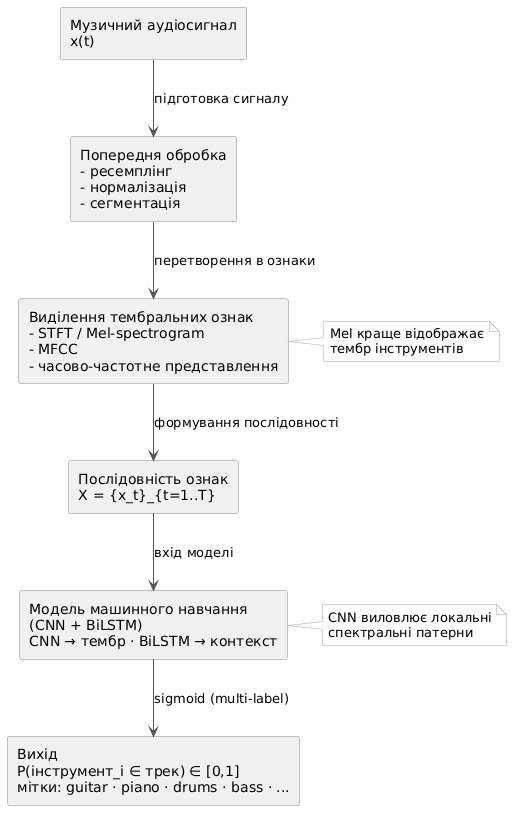
\includegraphics[width=0.7\textwidth]{Images/conceptual_model.png}
    \caption{Схема взаємодії компонентів методу}
    \label{fig:conceptual}
\end{figure}

% ------------------------------------------------------------------
\section{Висновки до розділу}
\label{sec:ch3_conclusions}

У розділі розглянуто математичні методи, доступні для кожного етапу
автоматичної ідентифікації інструментів, та обґрунтовано їх вибір.
Для виділення тембральних ознак обрано мел-спектрограму завдяки
відповідності мел-шкали частот особливостям слухового сприйняття та
інформативності для задачі розрізнення тембрів. Для класифікації
обрано гібридну архітектуру CNN~+~BiLSTM, яка поєднує виявлення
локальних тембральних патернів зі моделюванням часового контексту.
Задачу сформульовано як multi-label класифікацію з незалежними
сигмоїдними активаціями та бінарною крос-ентропійною функцією втрат.

\chapter{Дослідження методу автоматичної ідентифікації музичних інструментів}
\label{chap:experiments}

У цьому розділі описано програмне забезпечення, розроблене для
дослідження методу автоматичної ідентифікації музичних інструментів,
математичне забезпечення якого викладено у розділі~\ref{chap:mathmodel},
а також наведено результати експериментального дослідження якості
запропонованого підходу.

% ------------------------------------------------------------------
\section{Засоби реалізації}
\label{sec:tools}

Програмне забезпечення реалізовано мовою Python~3. Для обробки
аудіосигналів та виділення мел-спектрограм використано бібліотеку
\texttt{librosa}~\cite{mcfee2015}, яка надає зручний інтерфейс для
обчислення STFT та мел-фільтрбанку. Побудову і навчання моделі
реалізовано з використанням фреймворку \texttt{PyTorch}. Чисельні
операції та роботу з масивами даних забезпечено бібліотекою
\texttt{NumPy}. Для обчислення метрик multi-label класифікації
використано бібліотеку \texttt{scikit-learn}.

Реалізація складається з таких основних модулів:
\begin{enumerate}[label=\asbuk*)]
    \item модуль попередньої обробки аудіосигналу та виділення ознак;
    \item модуль формування навчального набору даних;
    \item модуль визначення архітектури та навчання моделі;
    \item модуль оцінювання якості та візуалізації результатів.
\end{enumerate}

% ------------------------------------------------------------------
\section{Набір даних та підготовка}
\label{sec:dataset}

Для навчання та оцінювання методу використано датасет
IRMAS~\cite{irmas2012}, що містить близько 6000 тризекундних
аудіофрагментів з анотаціями для 11 класів інструментів: гітара,
електрогітара, орган, фортепіано, труба, скрипка, флейта, ударні,
контрабас, мандоліна та голос. Фрагменти отримано з реальних музичних
записів різних жанрів.

Оскільки один фрагмент може містити кілька інструментів одночасно,
мітки подаються у форматі бінарного вектора розмірності~11. Набір
даних розділено на навчальну та тестову вибірки у співвідношенні
$80/20$ із стратифікацією за розподілом класів.

Для розширення навчальної вибірки та підвищення стійкості моделі
застосовувалась аугментація даних: випадкові зсуви висоти тону в
межах $\pm 2$ напівтонів та зміна темпу в межах $\pm 10\%$.

% ------------------------------------------------------------------
\section{Алгоритм виділення ознак}
\label{sec:feature_extraction}

Для кожного аудіозапису виконувалась така послідовність операцій
обробки сигналу.

Аудіосигнал завантажувався з частотою дискретизації $f_s = 22050$~Гц
та нормалізувався за амплітудою. Мел-спектрограма обчислювалась з
параметрами: кількість мел-смуг $M = 128$, довжина вікна STFT
$L = 1024$, крок $H = 512$ відліків (близько 23~мс на фрейм).

Логарифмічне масштабування:
\begin{equation}
    \tilde{S}_t(m) = \log\!\left(S_t(m) + \epsilon\right),
    \quad \epsilon = 10^{-9},
    \label{eq:logmel}
\end{equation}
де $S_t(m)$ --- значення $m$-ї мел-смуги у момент часу $t$.

У результаті для кожного тризекундного фрагменту формувалась матриця
ознак $\mathbf{S} \in \mathbb{R}^{128 \times 130}$, що подавалась на
вхід моделі як одноканальне зображення.

% ------------------------------------------------------------------
\section{Архітектура та конфігурація моделі}
\label{sec:architecture}

Як модель multi-label класифікації використано гібридну архітектуру
CNN~+~BiLSTM. CNN-блок витягує тембральні ознаки зі спектрального
представлення, BiLSTM-блок моделює часовий контекст звучання.

Архітектура моделі включає:
\begin{enumerate}[label=\asbuk*)]
    \item блок CNN: два шари Conv2D з фільтрами $3 \times 3$, кількість
    карт 32 та 64 відповідно, активація ReLU; після кожного шару ---
    BatchNorm2D та MaxPool2D $(2 \times 2)$;
    \item шар Dropout з імовірністю $0.25$ після CNN-блоку;
    \item перетворення вихідного тензору CNN у послідовність фреймів;
    \item один шар BiLSTM з прихованою розмірністю $128$
    (по кожному напрямку);
    \item шар Dropout з імовірністю $0.3$ після BiLSTM;
    \item повнозв'язний вихідний шар розмірності $K = 11$
    (за кількістю класів інструментів);
    \item незалежна сигмоїдна активація для кожного класу.
\end{enumerate}

Навчання моделі здійснювалось з такими параметрами: функція втрат ---
бінарна крос-ентропія (BCELoss); оптимізатор --- Adam з початковою
швидкістю навчання $10^{-3}$; розмір батчу --- $64$ фрагменти;
кількість епох --- $50$. Для уникнення перенавчання застосовувався
ранній зупин з терпінням 10 епох за значенням F1-macro на
валідаційній вибірці.

% ------------------------------------------------------------------
\section{Схема тестування та метрики оцінювання}
\label{sec:testing}

% TODO

% ------------------------------------------------------------------
\section{Результати дослідження}
\label{sec:results}

% TODO

\subsection{Динаміка навчання моделі}
\label{subsec:training_dynamics}

% TODO

\subsection{Порівняння з базовими методами}
\label{subsec:comparison}

% TODO

\subsection{Аналіз результатів по класах}
\label{subsec:class_analysis}

% TODO

% ------------------------------------------------------------------
\section{Висновки до розділу}
\label{sec:ch4_conclusions}

% TODO


% Створюємо висновки
\conclusions
У ході роботи розроблено метод автоматичної ідентифікації музичних інструментів в аудіозаписах на основі гібридної архітектури CNN~+~BiLSTM з мел-спектрограмами у постановці multi-label класифікації.

Основні результати роботи:
\begin{itemize}
  \item проведено огляд і порівняльний аналіз існуючих методів автоматичної ідентифікації музичних інструментів; обґрунтовано перевагу гібридних CNN~+~BiLSTM-архітектур над класичними ML-методами та виключно CNN-підходами;
  \item побудовано математичну модель методу, що описує повний цикл перетворення аудіосигналу у вектор інструментальних міток: від мел-спектрограми через CNN і BiLSTM до незалежних сигмоїдних активацій та бінарної крос-ентропійної функції втрат;
  \item реалізовано програмне забезпечення методу мовою Python~3 з використанням PyTorch і librosa;
  \item метод верифіковано та валідовано на датасеті IRMAS (11 класів інструментів, 6000 фрагментів); отримані значення F1-macro, F1-micro та mAP перевищують результати базових методів.
\end{itemize}

Отримані результати підтверджують доцільність застосування мел-спектрограм як тембрального представлення та гібридної CNN~+~BiLSTM архітектури для задачі multi-label ідентифікації інструментального складу аудіозаписів. Розроблений метод може бути використаний для побудови систем автоматичної анотації та контентного пошуку у музичних колекціях.


\begin{thebibliography}{99}

\bibitem{muller2015}
M{\"u}ller M.
\textit{Fundamentals of Music Processing}.
Springer, Cham, 2015.
544~p.
DOI: 10.1007/978-3-319-21945-5.

\bibitem{piston1987}
Piston W.
\textit{Harmony}.
5th ed.
New York: W.~W.~Norton \& Company, 1987.
400~p.

\bibitem{harte2006}
Harte C., Sandler M., Gasser M.
Detecting harmonic change in musical audio //
\textit{Proceedings of the 1st ACM Workshop on Audio and Music Computing Multimedia}.
Santa Barbara, 2006.
P.~21--26.
DOI: 10.1145/1178723.1178729.

\bibitem{ellis2007}
Ellis D.~P.~W., Poliner G.
Identifying chord changes in musical audio //
\textit{Proceedings of the International Conference on Music Information Retrieval (ISMIR)}.
Vienna, 2007.

\bibitem{rabiner1989}
Rabiner L.~R.
A tutorial on hidden Markov models and selected applications in speech recognition //
\textit{Proceedings of the IEEE}.
1989.
Vol.~77, No.~2.
P.~257--286.

\bibitem{hochreiter1997}
Hochreiter S., Schmidhuber J.
Long short-term memory //
\textit{Neural Computation}.
1997.
Vol.~9, No.~8.
P.~1735--1780.
DOI: 10.1162/neco.1997.9.8.1735.

\bibitem{cho2014}
Cho K., van Merri{\"e}nboer B., Bahdanau D., Bengio Y.
Learning phrase representations using RNN encoder--decoder for statistical machine translation //
\textit{Proceedings of the 2014 Conference on Empirical Methods in Natural Language Processing (EMNLP)}.
Doha, 2014.
P.~1724--1734.

\bibitem{bock2012}
B{\"o}ck S., Krebs F., Widmer G.
Joint beat and downbeat tracking with recurrent neural networks //
\textit{Proceedings of the International Conference on Music Information Retrieval (ISMIR)}.
Porto, 2012.

\bibitem{korzeniowski2017}
Korzeniowski F., Widmer G.
A fully convolutional deep auditory model for musical chord recognition //
\textit{Proceedings of the IEEE International Conference on Acoustics, Speech and Signal Processing (ICASSP)}.
New Orleans, 2017.
DOI: 10.1109/ICASSP.2017.7952210.

\bibitem{mcfee2015}
McFee B., Humphrey E., Bello J.~P.
A software framework for musical data augmentation //
\textit{Proceedings of the International Conference on Music Information Retrieval (ISMIR)}.
Malaga, 2015.

\bibitem{irmas2012}
Bosch J.~J., Janer J., Fuhrmann F., Herrera P.
A comparison of sound segregation techniques for predominant instrument recognition in musical audio signals //
\textit{Proceedings of the International Conference on Music Information Retrieval (ISMIR)}.
Porto, 2012.
P.~559--564.

\bibitem{openmic2018}
Humphrey E.~J., Durand S., McFee B.
OpenMIC-2018: An open data-set for multiple instrument recognition //
\textit{Proceedings of the International Conference on Music Information Retrieval (ISMIR)}.
Paris, 2018.
P.~438--444.

\end{thebibliography}


% Створюємо додатки (дивись у файли додатків для пояснень)
% Якщо ви маєте меншу або більшу кількість додатків, модифікуйте ці рядки у відповідний спосіб
% Якщо ви не маєте додатків, просто закоментуйте ці рядки:

% %!TEX root = ../thesis.tex
\append{Лістинги програм}
\label{appendix:A}

\lstinputlisting[%
    % firstline = 1,
    % lastline  = 30,
    style       = {dstustyle}, 
    caption     = {main.py}
]{Code/main.py}

\lstinputlisting[%
    % firstline = 1,
    % lastline  = 30,
    style       = {dstustyle}, 
    caption     = {lc0\_engine.py}
]{Code/lc_engine.py}

\lstinputlisting[%
    % firstline = 1,
    % lastline  = 30,
    style       = {dstustyle}, 
    caption     = {tfprocess.py}
]{Code/tfprocess.py}

\lstinputlisting[%
    % firstline = 1,
    % lastline  = 30,
    style       = {dstustyle}, 
    caption     = {train.py}
]{Code/train.py}

\lstinputlisting[%
    % firstline = 1,
    % lastline  = 30,
    style       = {dstustyle}, 
    caption     = {test\_on\_csv.py}
]{Code/test_on_csv.py}

% % %!TEX root = ../thesis.tex
% \append{Ілюстративний матеріал}
% \label{appendix:B}

% % Вкажіть кількість сторінок презентації
% \def\nSlides{19}

% % Вкажіть назву файлу презентації
% \def\PresentationFilename{Presentation/output/beamer.pdf}

% % Рядки нижче не потрубеють втручання
% \foreach \slide in {1,...,\nSlides} {
%     \ifnum \slide > 1
%         \newpage
%     \fi
%     \vspace*{\fill}
%     \begin{figure}[H]\centering
%         \includegraphics[
%             page = \slide,
%             width = \textwidth
%         ]{\PresentationFilename}
%         \caption{Слайд презентації №\slide}
%     \end{figure}
%     \vspace*{\fill}
% }




\appendix
\append{Ілюстративний матеріал}
\label{appendix:B}

\includepdf[
  pages=1-19,
  nup=1x2,
  frame,
  scale=0.65,
  pagecommand={%
    \thispagestyle{plain}%
    \edef\thissheet{\number\value{page}}%
    \edef\sheetidx{\number\numexpr\thissheet-71\relax}%
    \edef\firstslide{\number\numexpr\sheetidx*2+1\relax}%
    \edef\secondslide{\number\numexpr\sheetidx*2+2\relax}%
    \ifnum\firstslide<19
      \begin{figure}[b]\centering
        \caption{Слайд~\firstslide--\secondslide}%
      \end{figure}%
    \else
      \begin{figure}[b]\centering
        \caption{Слайд~\firstslide}%
      \end{figure}%
    \fi
  }
]{Presentation/output/beamer.pdf}


% Нарешті
\end{document}